\chapter{Testing. Existing approaches. Test Sheets}
\section{Software testing}
%Oxford dictionary defines test as a procedure intended to establish the quality, performance, or reliability of something, especially before it is taken into widespread use. 
Software testing is an important technique to evaluate and assess software's quality and reliability, it provides possibility to determine whether the development of product conform the requirements. The variety of tests coincides the variety of requirements for the software under test. At least 30\% of the price of software project is the cost of software testing \cite{Lecture2}. 
A General requirements to test definitions are following: fast, independent, repeatable, self-validating, timely.
More detailed information regarding requirements can be found via following URL: \url{http://www.extremeprogramming.org/rules/testfirst.html}
 %The price of software project for at least 30\% consists of costs for tests\cite{Lecture2}.
%The knowledge on software testing have become crucial for all software developers and engineers\cite{IntroductionST}.
%Robert Cecil Martin in his book 'Clean Code: A Handbook of Agile Software Craftsmanship'\cite{MartinClean} says following: "Tests are as important to the health of a project as the production code is. Perhaps they are even more important, because tests preserve and enhance the flexibility, maintainability, and reusability of the production code."
%"Test processes determine whether the development products of a given activity conform to the requirements of that activity and whether the system and/or software satisfies its intended use and user needs. Testing process tasks are specified for different integrity levels. These process tasks determine the appropriate breadth and depth of test documentation. The documentation elements for each type of test documentation can then be selected. The scope of testing encompasses software-based systems, computer software, hardware and their interfaces. This standard applies to software-based systems being developed, maintained, or reused (legacy, COTS, Non-Developmental Items). The term software also includes firmware, microcode and documentation. Test processes can include inspection, analysis, demonstration, verification and validation of software products."\cite{draft}
\paragraph{The economical costs} of unexpected software behavior (bug, failure or error) can go up to several millions or even billions of USD. \\
\textit{\textbf{Web application failures}} only in USA lead to looses of \$6.5 million per hour in financial services and \$2.4 million per hour in credit card sales applications\cite{Lecture1}. \\
\textit{\textbf{Alarm-management}} fault was one of the reasons of the black-out occurred in the northeastern US on August 2003. Estimated costs were between US\$7 and \$10 billion\cite{costOfErrors}.\\
\textit{\textbf{In general,}} according to report made by US National Institute of Standards and Technology (NIST) in 2009 the estimated economy loses  were \$60 billion anually as associated with developing and distributing software patches and reinstalling systems that have been involved, together with losses in productivity due to errors and malware infections\cite{costOfErrors}.\\


%\paragraph{The human causalities} caused by software misbehavior can rich dramatic scales.\\
%\textit{\textbf{The case of Toyota}} unintended acceleration caused by software defect  in 2009 - 2011 led to 89 deaths and 57 injures.
%Toyota was fined \$1.2 Billion for concealing safety defects\cite{toyota}.\\
%\textit{\textbf{The Patriot,}} surface-to-air missile, system failed to track and intercept an incoming Scud missile on 25 of February 1991. As the result 28 soldiers were killed and around 100 were injured\cite{costOfErrors}.\\
%\textit{\textbf{A Therac-25}}, linear accelerator, which failure caused to 6 know cases where cancer patients received deadly radiation overdoses during their treatment between June 1985 and January 1987. The dosages were 100 times exceeding typically used for treatment\cite{costOfErrors}\cite{therac}.\\

%The variety of tests coincides the variety of requirements for the software under test. Test processes determine whether the software conform to the requirements and/or satisfies its intended use and user needs\cite{ieeeTesting}. As well as this is an important technique to evaluate and help to improve software quality, reliability and saftiness\cite{cota}.





%This led to new requirements for testing definition and representation tools since old tools like JUnit have high entry level for test engineers and requires its users to have an ability to write and read an executable code in a corresponding programming language.




%According to IEEE Standard for Software and System Test Documentation the process of software testing includes "inspection, analysis, demonstration, verification, and validation".

%"Test processes determine whether the development products of a given activity conform to the requirements of that activity and whether the system and/or software satisfies its intended use and user needs. Testing process tasks are specified for different integrity levels. These process tasks determine the appropriate breadth and depth of test documentation. The documentation elements for each type of test documentation can then be selected. The scope of testing encompasses software-based systems, computer software, hardware, and their interfaces. This standard applies to software-based systems being developed, maintained, or reused (legacy, commercial off-the-shelf, Non-Developmental Items). The term "software" also includes firmware, microcode, and documentation. Test processes can include inspection, analysis, demonstration, verification, and validation of software and software-based system products."\cite{ieeeTesting}


%"Software testing has grown as an important technique to evaluate and help to improve software quality.
%Numerous techniques and tools have appeared in the last decade, ranging from static analysis to automatic test generation and application.
%One can argue that software is the dominant part of an embedded system, either as a final product (executable code) or during its development lifecycle (system modeling in specific languages and computation models).
%In both cases, software must be thoroughly verified to ensure product quality and reliability.
%One can observe a growing number of academic and industrial works on the topic of embedded SW testing in the last four or five years, and this seems to be a good time for reflection: how exactly is embedded software testing different from traditional software testing? 
%Is it an engineering or computer science problem? 
%Does it need extra support from platform developers? 
%What is the role of the SW engineer and of the designer in developing a high-quality software-based embedded application?
%Many authors suggest that, on top of the ordinary software testing challenges, software usage in an embedded application brings additional issues that must be dealt with: the variety of possible target platforms, the different computational models involved during the design, faster time-to-market and even more instable and complex specifications, platform-dependent constraints (power, memory, and resources availability), etc.
%On the other hand, current platforms are more and more powerful, and the specificities of the embedded application can help to reduce the search space during test generation:
%application domains, strong code reuse paradigm, use of less advanced programming language resources, and common availability of system models subject to or already verified with respect to specific properties, for instance.
%Furthermore, a major part of the so-called embedded software does not depend directly on hardware, and one can argue that only a small percentage really needs to be tested together with the target platform, and this test is part of the platform design, not the system design. "\cite{cota}

%Introduction of Agile and Extreme development paradigms with increased requirements for control over the existing code, its reuse and maintenance lifted requirements for tests and their quality to the new level and shifted responsibility regarding testing process from software engineers to people without development background. 
%This led to new requirements for testing definition and representation tools since old tools like JUnit have high entry level for test engineers and requires its users to have an ability to write and read an executable code in a corresponding programming language.

\section{Existing approaches for test definitions}
In most of the cases developers are using testing frameworks or internal DSLs which requires usage of formal programming languages. This in a result makes writing of tests not different from the programming. It requires knowledge of languages and understanding of basic programming concepts from everyone who is involved in the creation of a test, reading its result or updating/deleting the test.
Since it is common practice to base tests on top of business requirements tests should be used by different shareholders who define this requirements.
Below provided brief overview of different testing approaches and their analysis with respect to modern business requirements.

\subsection{xUnit}
xUnit is a family of unit testing frameworks with shared architecture and functionality which is derived from Smalltalk's SUnit, designed for tests automation\cite{xunit}\cite{xunitFowler}. The general simplicity and lightweight made them popular tool for Test Driven Development\cite{xunitFowler}.

xUnit basic features implemented by all members of the family provide functionality to perform following tasks\cite{xunit}:
\begin{enumerate}
	\item Specify a test as a \textit{Test Method};
	\item Specify the expected results within the test method in the form of calls to \textit{Assertion Methods};
	\item Aggregate the tests into test suites that can be run as a single operation;
	\item Run one or more tests to get a report on the results of the test run
\end{enumerate}

Test \textbf{\textit{cases}} in xUnit are defined as a methods united in to \textbf{\textit{suites}} with shared preconditions called \textbf{\textit{fixtures}}.  Cases or suites are executed by a \textbf{\textit{runner}} which compares actual and expected results using \textbf{\textit{assertion}} function.

The family includes a wide variety of implementations for multiple programming languages, and diverse enhancement of functionality (e. g. code coverage statistics, assertion add-ons etc.)\cite{xunitWiki}.

Definition of tests with formal general programming language from one side makes tests definition and execution fast but in a same time makes impossible the creation of tests for people without developer background. 

\subsection{Fit}
Framework for Integrated Test (Fit) - is a way of defining test cases with HTML pages. It enhances the communication and collaboration connecting customers and programmers. Moreover, it creates feedback loop between them. Fit automatically checks HTML pages against actual program\cite{fit}.

Fit reads tables in HTML files, each table is interpreted by a \textit{fixture} written by programmers. This fixture checks the examples in the table by running the actual program\cite{fitIntro}.

Programmers use a \textit{ColumnFixture} to map the columns in the table to variables and methods in the fixture. The first columns provide correspond to variables in the fixture. The last column has the expected result and corresponds to the method in the fixture\cite{fitIntro}.

Different implementation provide different user experience from Wiki pages (i.e. FitNess) to complete standalone application with internal functionality for tables definitions and tests execution (i.e. GuiRunner).

With Fit, customers can provide more guidance in a development process by lending their subject matter expertise and imagination to the effort\cite{fit} requiring developer to write only \textit{fixture}, the middleware between tests and code. In the same time it provides media between  CRUD operations over tests and the results of their execution for people without development experience.

\subsection{Cucumber}
Cucumber is a Behavior Driven Development tool which allows users to define tests specifications with \textit{Gherkin}, the language which is structured plain text with support of internationalization for 60+ different languages\cite{cuceRef}.

Feature files written in Gherkin consists of plain text and general key-words are used for identification of following concepts:
\begin{itemize}
	\item Feature under the test: \textit{Feature};
	\item Test scenario: \textit{Scenario};
	\item Scenario Outline: \textit{Scenario Outline}
	\item Test Steps: \textit{Given, When, Then, And, But};
	\item Test Background:  \textit{Background};
	\item Test Examples: \textit{Examples}
\end{itemize}

Specific characters are used for identification of:
\begin{itemize}
	\item Step Inputs: String - \textit{"""}, Table - \textit{$|$};
	\item Step Tags: \textit{@};
	\item Comments: \textit{\#}
\end{itemize}

Step definitions are written by developers. Definition parses feature file with attached pattern to link all the step matches and code executed by cucumber when match is met.

Human readable input and output of the tests defined in gherkin makes cucumber a good media for communication between people who create requirements and those who are trying to meet them. But in a same time software development experience required for writing code with step definitions.

\section{Test Sheets}
Test Sheets is a representation for tests a developed with the goal to combine the power and completeness of formal programming language with a representation that is easy to understand and work with even for people with little IT knowledge\cite{ts}.

Test Sheets approach uses usual spreadsheet for definition of test and representation of their result. 
\begin{itemize}
	\item Rows - represent operations being executed;
	\item Columns -  variables for input or output parameters;
\end{itemize}

The actual content of a cell can be made dependent on other cells by addressing them via their location.
Just like in Fit result of tests execution is provided in a same table with coloring and actual return are separated by "\textbackslash"\ symbol in case of failing test\cite{tsb}.

There are three types of test sheets which can be used in combination:
\begin{itemize}
	\item \textbf{Basic} - order of test step execution is defined by order of rows in a table;
	\item \textbf{Non-Linear} - order of test steps execution is defined by finite state machine with states represented by test steps and transition function by step execution results or number of test step execution;
	\item \textbf{High-Order/Parametrized} - The actual value used for Parameterized Test Sheets is specified by a Higher-Order Test Sheet in a column with letter Parametrized Test Sheet refers to.
\end{itemize}
The main benefit of this approach over \textit{xUnit}, \textit{Cucumber}, \textit{Fit} is an exclusion of software developers from CRUD test operations which can be performed by user without prior development experience with usage of any spreadsheet editor.

 \subsection{Basic Test Sheets}
A Basic Test Sheet is a type of Test Sheets with sequential tests execution without parametrized values, but with possibility to use references between cells for definition of values.
The rows content is structured as following:
\begin{itemize}
	\item \textit{Test name} - first row;
	\item \textit{Class/Module under test} - second row;
	\item \textit{Test step} - all next rows represent method calls;
\end{itemize}

Values in columns cells of which belong to the test step has net purposes:
\begin{itemize}
	\item \textit{Object Under Test} - cells in a first column;
	\item \textit{Method Under Test} - cells in a second column;
	\item \textit{Input Parameters} - cells in a next column before invocation line;
	\item \textit{Invocation Line} - cells in a delimiter column between cell(s) with biggest number of input and column with expected return value;
	\item \textit{Expected Return} - cells in a column after invocation line;
\end{itemize}

The description provided above is shown in a summarized example from the web site of Chair of Software Engineering of University of Mannheim (Pic.: \ref{fig:BasictestSheet}).
  \begin{figure}[ht]
  	\label{fig:BasictestSheet}
    \centering
    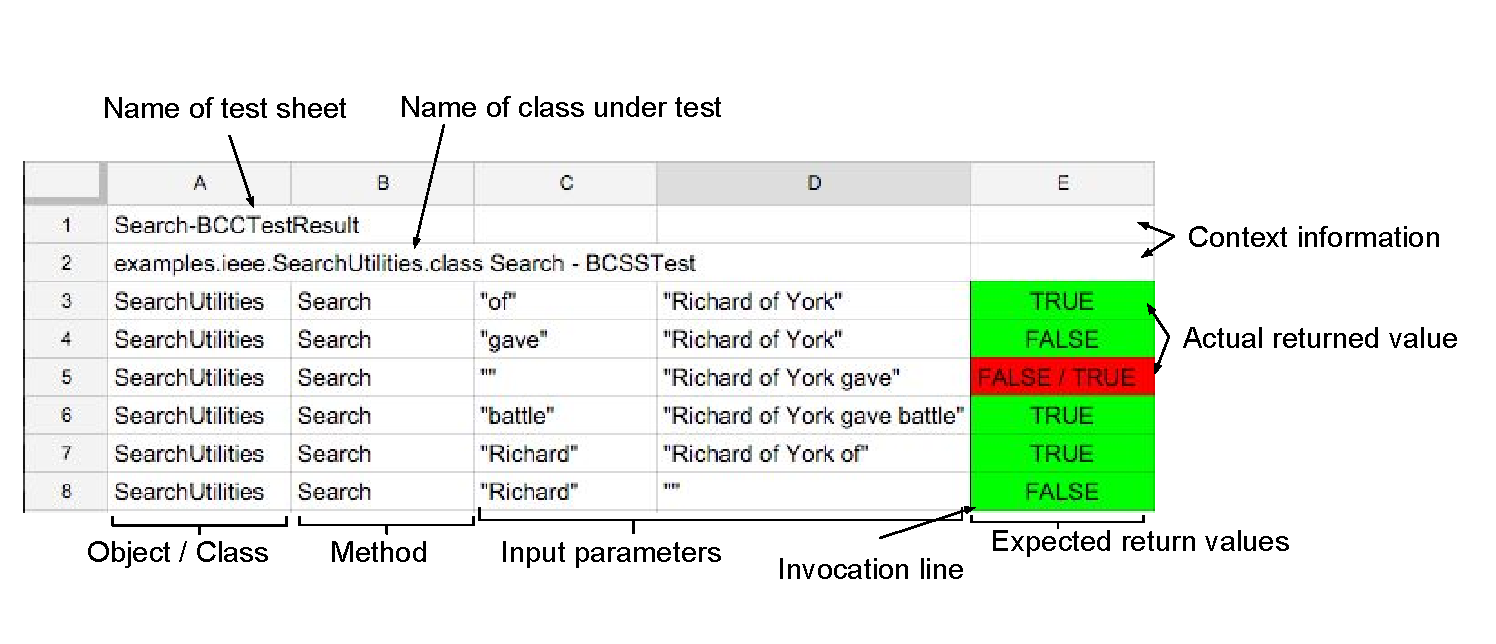
\includegraphics[width=\textwidth]{grafiken/basic_test_sheet}
     \caption{Basic Test Sheet}
  \end{figure}



The software developed within the scope of this research is a proof of concept for an usage of Test Sheets for scenario testing of asynchronous real-time software. The scope of this paper covers only Basic Test Sheets. For more details about Test Sheets and Research Topics of the Chair of Software Engineering please visit \url{http://swt.informatik.uni-mannheim.de/de/home/}.

% \paragraph{Non-Linear}
%Similar to the invocation line (double line separating input parameters and expected return values) there is a double line below the last method invocation row.
%Below this line the behavior specification starts. 
%Each row of the behavior specification represents a state of a state machine. 
%The state machine starts in the first state that is being specified right below the double line and stops execution once a state is reached without any valid transitions.

%Each column in a row specifies a transition. 
%A transition consists of a guard, executed invocations and a subsequent state. 
%The starting state has only one transition with no guard, the intermediate state has [...] transitions each with a guard and the terminating state does not have any transitions at all[...].  \cite{tsn}

%\section{High Order, Parameterized Test Sheets}
%"The actual value used for Parameterized Test Sheets is specified by a Higher-Order Test Sheet as in the example below. 
%The Higher-Order Test Sheet references the Parameterized Test Sheet as the 'class' being tested. 
%On said pseudo-class it invokes the pseudo-method test followed the by the value to be used as parameter. 
%?C in the Parameterized Test Sheet is replaced by the value defined the third column (column C) for each execution.
%It is also possible to use more than one parameter. These are defined in the Higher-Order Test Sheet in subsequent columns (D, E, F, etc.) and referenced in the Parameterized Test Sheet via ?D, ?E, ?F, etc"\cite{tsh}
